
%(BEGIN_QUESTION)
% Copyright 2013, Tony R. Kuphaldt, released under the Creative Commons Attribution License (v 1.0)
% This means you may do almost anything with this work of mine, so long as you give me proper credit

Examine this process trend showing the PV, SP, and Output of a loop controller:

$$\includegraphics[width=15.5cm]{i02638x01.eps}$$

Based on what you see here, determine the following:

\begin{itemize}
\item{} Whether this is an open-loop or a closed-loop response
\item{} Whether the controller is (or needs to be) {\it direct-acting} or {\it reverse-acting}
\item{} If possible, identify any problems with the field instrumentation
\item{} If possible, identify any problems with the controller PID tuning
\item{} Qualitatively identify the kind of PID tuning we will need for robust control
\end{itemize}

\underbar{file i02638}
%(END_QUESTION)





%(BEGIN_ANSWER)

This is a {\it closed-loop test}, based on the fact the output signal responds dynamically to the changing process variable, as well as to the step-change in setpoint.

\vskip 10pt

This is a {\it reverse-acting} controller: the output steps up when the setpoint steps up (implying the output would step down if the process variable stepped up).

\vskip 10pt

The only problem here is that the process exhibits a varying gain.  This is why the control is over-sensitive (oscillatory) at high setpoint values and sluggish at low setpoint values.  This could be a function of process dynamics, or of a control valve with the wrong characteristic (e.g. an equal-percentage valve in an application better suited for a linear valve).

\vskip 10pt
  
The controller tuning looks really good when the process variable is maintaining around 40\%.  This mid-range is where the tuning seems to be optimized.  

\vskip 10pt

This process appears to be self-regulating with short dead and lag times.  It is clear from examining the phase shifts of output versus PV that there is some derivative action at work here, since the output actually leads the PV when there is oscillation.  The key will be linearizing the process gain so that one set of tuning parameters will work robustly across the control range.

%(END_ANSWER)





%(BEGIN_NOTES)


%INDEX% Process troubleshooting: diagnosing problem via trend recording

%(END_NOTES)


